% In your .tex file
% !TEX program = latex
%  A simple AAU report template.
%  2014-09-13 v. 1.1.0
%  Copyright 2010-2014 by Jesper Kjær Nielsen <jkn@es.aau.dk>
%
%  This is free software: you can redistribute it and/or modify
%  it under the terms of the GNU General Public License as published by
%  the Free Software Foundation, either version 3 of the License, or
%  (at your option) any later version.
%
%  This is distributed in the hope that it will be useful,
		%  but WITHOUT ANY WARRANTY; without even the implied warranty of
%  MERCHANTABILITY or FITNESS FOR A PARTICULAR PURPOSE.  See the
%  GNU General Public License for more details.
%
%  You can find the GNU General Public License at <http://www.gnu.org/licenses/>.
%
%  A simple AAU report template.
%  2014-09-13 v. 1.1.0
%  Copyright 2010-2014 by Jesper Kjær Nielsen <jkn@es.aau.dk>
%
%  This is free software: you can redistribute it and/or modify
%  it under the terms of the GNU General Public License as published by
%  the Free Software Foundation, either version 3 of the License, or
%  (at your option) any later version.
%
%  This is distributed in the hope that it will be useful,
%  but WITHOUT ANY WARRANTY; without even the implied warranty of
%  MERCHANTABILITY or FITNESS FOR A PARTICULAR PURPOSE.  See the
%  GNU General Public License for more details.
%
%  You can find the GNU General Public License at <http://www.gnu.org/licenses/>.
%
\documentclass[11pt,a4paper,openleft,final,oneside]{memoir}
\usepackage{etex}
%%%%%%%%%%%%%%%%%%%%%%%%%%
%% COMMAND DEACTIVATION %%
%%%%%%%%%%%%%%%%%%%%%%%%%%

\let\added\undefined
\let\deleted\undefined


%%%%%%%%%%%%%%
%% PACKAGES %%
%%%%%%%%%%%%%%


%%% Initial things %%%
% Fix various issues with LaTeX2e
\usepackage{fixltx2e}
% Font package
\usepackage{fourier}
% Index
\usepackage{makeidx}
\makeindex


%%% Translations and character encodings %%%
% Enable use of several characters, including æ, ø and å
\usepackage[utf8]{inputenc}
%  language
\usepackage[english]{babel}
% Use PostScript fonts instead of bitmap ones. Also does other stuff.
\usepackage[T1]{fontenc}
% Various LaTeX symbols
\usepackage{latexsym}
% Wider selection of colours
\usepackage[pdftex,dvipsnames,table]{xcolor}  % Coloured text etc.% Improved element justification
\usepackage{ragged2e}
% Font improvements
\usepackage{fix-cm}
% Enables inclusion of PDF files
\usepackage{pdfpages}
% Enables various forms of lines, like double-underlining (\uuline{})
\usepackage[normalem,normalbf]{ulem}
% Sets the tolerance for distance between words, determining when to hyphenate.
\pretolerance=2500


%%% Figures and tables (Floats) %%%
% Ensures that floats won't appear -before- the place where they're added
\usepackage{flafter}
% Enable multi-rows and -columns
\usepackage{multirow}
\usepackage{multicol}
% Double, horizontal lines
\usepackage{hhline}
% Enables coloured tables
\usepackage{colortbl}
% Gives improved control over placement of floats
% \begin{figure}[!h] % Won't be floating
\usepackage{here}
% Wrap text around figures
\usepackage{wrapfig}
% Wrap text around tables
\usepackage{floatflt}
% Enables the \FloatBarrier command
\usepackage{placeins}
% Rotation of figures
\usepackage{rotating}
% Framed boxes
\usepackage{framed}
% Booktabs - Fancy tables
\usepackage{booktabs}
% Enables inclusion of PDF documents of version 1.6+
%\pdfoptionpdfminorversion=6 
\usepackage{tabularx}


%%% Mathematic formulas %%%
% AMS math
%\usepackage{amsmath}
%\usepackage{amssymb}
% Extra fonts (for math, I think)
\usepackage{stmaryrd}
% Access text symbols
\usepackage{textcomp}
% Extend AMS
%\usepackage{mathtools}
%\usepackage{cancel}
% Use theorems in your document
% The ntheorem package is also used for the example environment
% When using thmmarks, amsmath must be an option as well. Otherwise \eqref doesn't work anymore.
%\usepackage[framed,amsmath,thmmarks]{ntheorem}
% Pretty fractions, just because
%\usepackage{nicefrac}


%%% Graphics %%%
% Various image-commands
\usepackage{eso-pic}
% Use JPEG and PNG images
\usepackage{array,graphicx}
\DeclareGraphicsExtensions{.pdf,.png,.jpg}
\graphicspath{{./images/}}
%Wrapping Images
\usepackage{wrapfig}


%%% Text stuff %%%
% Filler text
%\usepackage{lipsum}
% Page counting
%\usepackage{totpages}
% Acronyms
%\usepackage{acronym}
%avoid widows
%\widowpenalty10000


%%% Source Code Stuff %%%
% Adds \lstinline!code there!, where !! are delimeters not used in the code
% Adds the environment: lstlisting
% Adds command \lstinputlisting[options]{filename.ext}
% More info in manual.
%\usepackage{listings}
%\lstloadlanguages{[Sharp]C,XML,SQL}
%\lstset{numbers=left,
%        numberstyle=\tiny,
%        stepnumber=2,
%        numbersep=5pt,
%        frame=tb,
%        inputencoding=utf8,
%        tabsize=2,
%        extendedchars=true,
%        language=[Sharp]C}



\usepackage{color}
\definecolor{bluekeywords}{rgb}{0.13,0.13,1}
\definecolor{greencomments}{rgb}{0,0.5,0}
\definecolor{redstrings}{rgb}{0.9,0,0}

\definecolor{mygreen}{rgb}{0,0.6,0}
\definecolor{mygray}{rgb}{0.5,0.5,0.5}
\definecolor{mymauve}{rgb}{0.58,0,0.82}

\usepackage{courier}

\usepackage{listings}


\lstset{ %
  backgroundcolor=\color{white},   % choose the background color; you must add \usepackage{color} or \usepackage{xcolor}
  basicstyle=\footnotesize,        % the size of the fonts that are used for the code
  breakatwhitespace=false,         % sets if automatic breaks should only happen at whitespace
  breaklines=true,                 % sets automatic line breaking
  captionpos=b,                    % sets the caption-position to bottom
  commentstyle=\color{mygreen},    % comment style
  deletekeywords={...},            % if you want to delete keywords from the given language
  escapeinside={\%*}{*)},          % if you want to add LaTeX within your code
  extendedchars=true,              % lets you use non-ASCII characters; for 8-bits encodings only, does not work with UTF-8
  frame=single,                    % adds a frame around the code
  keepspaces=true,                 % keeps spaces in text, useful for keeping indentation of code (possibly needs columns=flexible)
  keywordstyle=\color{blue},       % keyword style
  language=java,                 % the language of the code
  otherkeywords={*,...,public, int16, int64, float64, float16, Void, Variable, Scope, String, foreach, ValueType},            % if you want to add more keywords to the set
  numbers=left,                    % where to put the line-numbers; possible values are (none, left, right)
  numbersep=5pt,                   % how far the line-numbers are from the code
  numberstyle=\tiny\color{mygray}, % the style that is used for the line-numbers
  rulecolor=\color{black},         % if not set, the frame-color may be changed on line-breaks within not-black text (e.g. comments (green here))
  showspaces=false,                % show spaces everywhere adding particular underscores; it overrides 'showstringspaces'
  showstringspaces=false,          % underline spaces within strings only
  showtabs=false,                  % show tabs within strings adding particular underscores
  stepnumber=1,                    % the step between two line-numbers. If it's 1, each line will be numbered
  stringstyle=\color{mymauve},     % string literal style
  tabsize=2,                       % sets default tabsize to 2 spaces
  title=\lstname,                   % show the filename of files included with \lstinputlisting; also try caption instead of title
    literate={ø}{{\o}}1
         {æ}{{\ae}}1
         {å}{{\aa}}1
         {Ø}{{\O}}1
         {Æ}{{\AE}}1
         {Å}{{\AA}}1
         {§}{{\S}}1
}

\lstdefinestyle{java}{
  belowcaptionskip=1\baselineskip,
  breakatwhitespace=false,        % sets if automatic breaks should only happen at whitespace
  breaklines=true,                % sets automatic line breaking
  xleftmargin=\parindent,
  language=Java,
  tabsize=4,
  numbers=left,                    % where to put the line-numbers; possible values are (none, left, right)
  numbersep=5pt,                   % how far the line-numbers are from the code
  numberstyle=\Tiny\color{mygray}, % the style that is used for the line-numbers
  showstringspaces=false,
  basicstyle=\footnotesize\ttfamily,
  keywordstyle=\bfseries\color[rgb]{.133,.545,.133},
  commentstyle=\itshape\color{blue},
  stringstyle=\color{mauve},
  directivestyle=\bfseries\color{purple},
  frame=single],
  resetmargins=true,
  morecomment=[s]{/*}{*/},
  morekeywords={public, int16, int64, float64, float16, Void, Variable, Scope, String, foreach},
  sensitive=true
}


\lstdefinestyle{make}{tabsize=4}

%%% References, bibtex and URLs %%%
% Post URLs. Allows breaking at hyphens to help avoid long links.
\usepackage[hyphens]{url}
% Better cross references
\usepackage[danish]{varioref}
% Enable natbib citation styles
\usepackage[numbers]{natbib}
% Define a new 'leo' style for URL package, that will use a smaller font
\makeatletter
\def\url@leostyle{%
  \@ifundefined{selectfont}{\def\UrlFont{\sf}}{\def\UrlFont{\small\ttfamily}}
}
\makeatother
% And of course, use this new style
\urlstyle{leo}




%%% Floats %%%
% Not entirely sure why I need this yet
\let\newfloat\relax
\usepackage{float}
% Enables usage of \subcaption, \subtop and \subbottom
\newsubfloat{figure}


%%% Todo Stuff %%%
% Insert needed corrections with \fixme{..}, which will cause an error during compile, if any are present once 'draft'
% is replaced with 'final'
\usepackage[footnote,english,silent,nomargin]{fixme}
\fxsetup{layout={footnote,marginclue,index},innerlayout={inline,index}}


%%% Changes Markup %%%
% Markup changes of varying types.
% Adds the commands:
%  - \added[id=(author id), remark={remark text}]{new text}
%  - \deleted[id=(author id), remark={remark text}]{old text}
%  - \replaced[id=(author id), remark={remark text}]{new text}{old text}
\usepackage[xcolor,authormarkup=footnote]{changes}
% Adds the commands:
%  - \cbstart
%  - \cbend
%  - \cbdelete
%  - Environment: changebar
\usepackage[outerbars,xcolor]{changebar}
\cbcolor{red}



%%%%%%%%%%%%%%%%%%%%%%%
%% DOCUMENT SETTINGS %%
%%%%%%%%%%%%%%%%%%%%%%%


%%% Margins %%%
% \setlrmarginsandblock{binding}{edge}{ratio}
\setlrmarginsandblock{2.0cm}{2.0cm}{*}
% \setulmarginsandblock{top}{bottom}{ratio}
\setulmarginsandblock{2.0cm}{2.0cm}{*}
% Performs various calculations and makes several non-Memoir things work with the Memoir class
\checkandfixthelayout 
% Correct todonotes placement
\reversemarginpar


%%% Paragraph formatting %%%
% Size of paragraph indentation
\setlength{\parindent}{0mm}
% Distance between paragraphs (double enter)
\setlength{\parskip}{3mm}
% Line distance
\linespread{1,1}


%%% Bibliography %%%
% Defines parameters for the bibliography, such as the parenthesis and separators
%%%% OLD STYLE!
%\bibpunct{[}{]}{,}{a}{}{;}
% Bibliography style
%%%% OLD STYLE!
%\bibliographystyle{bibtex/harvard}
\bibliographystyle{plain}
%\bibliographystyle{unsrt}


%%% Table of contents %%%
% Depth of numbered headlines
\setsecnumdepth{subsubsection}
% Changing the document class' limit for number-depth
\maxsecnumdepth{subsection}
% Define the depth included in the table of contents
\settocdepth{section}
% Use letters instead of Roman numerals in TOC
\renewcommand{\thepart}{\Alph{part}}


%%% Text stuff %%%
% Removes distance between items in itemize
%\let\olditemize=\itemize
%\def\itemize{\olditemize\setlength{\itemsep}{-1ex}}
%% Removes distance between items in enumerate
%\let\oldenumerate=\enumerate
%\def\enumerate{\oldenumerate\setlength{\itemsep}{-1ex}}
\usepackage{enumitem}
\usepackage{mdwlist}


%%% Changes (Language strings) %%%
\addto\captionsdanish{
  \def\listofchangesname{Ændringer i dokumentet}
  \def\summaryofchangesname{Ændringer}
  \def\changesaddname{Tilføjet}
  \def\changesdeletename{Slettet}
  \def\changesreplacename{Erstattet}
  \def\changesauthorname{Skribent}
  \def\changesanonymousname{anonym}
  \def\changesnoloc{Listen af ændringer tilgængelig efter næste \LaTeX\ kørsel.}
  \def\changesnosoc{Opsummering af ændringer tilgængelig efter næste \LaTeX\ kørsel.}
}


%%% Visual references %%%
% Enables clickable hyperlinks

%%% Add hidelinks to remove boxes around links

\usepackage[colorlinks,backref=page,hidelinks]{hyperref}
% General setup of hyperlinks package
\hypersetup{
    breaklinks = true,
    colorlinks = false,
    linkcolor = black,
    anchorcolor = black,
    citecolor = black
}


%%% Colour definitions %%%
% Defines: gray
\definecolor{gray}{gray}{0.80}
% Defines: numbercolor
\definecolor{numbercolor}{gray}{0.7}
% Defines: shadecolor
\definecolor{shadecolor}{RGB}{33,26,82}
% Defines: aaublue
\definecolor{aaublue}{RGB}{33,26,82}


%%% Figure and table texts setup %%%
% Font definition for the 'Figure' or 'Table' displays.
\captionnamefont{\small\bfseries\itshape}
% Font definition for the numbering
\captiontitlefont{\small}
% Delimiter between number and figure text
\captiondelim{. }
% Left justify multi-line figure texts below one another
\hangcaption
% Width of figure text
\captionwidth{\linewidth}
% Distance below figure text
\setlength{\belowcaptionskip}{10pt}
% Fix space between figure number and name
\setlength{\cftfigurenumwidth}{14mm}


%%% Page header and footer %%%
% Define width of header and footer
\setlength{\headwidth}{\textwidth}
% Create pagestyle for pages with and without a new chapter
\makepagestyle{reportPlain}
\makepagestyle{reportChapter}
% Pagestyle for chapter pages (Only a footer, of course)
\makefootrule{reportChapter}{\headwidth}{\normalrulethickness}{\footruleskip}
\makeevenfoot{reportChapter}{\thepage}{}{}
\makeoddfoot{reportChapter}{\thepage}{}{}

%\makeoddfoot{reportChapter}{}{}{\thepage}
% Pagestyle for regular pages
\makerunningwidth{reportPlain}{\headwidth}
\makeheadposition{reportPlain}{flushright}{flushleft}{flushright}{flushleft}
\makeevenhead{reportPlain}{\leftmark}{}{}
\makeoddhead{reportPlain}{}{}{\rightmark}
\makeevenfoot{reportPlain}{\thepage}{}{}
\makeoddfoot{reportPlain}{}{}{\thepage}
\makeheadrule{reportPlain}{\headwidth}{\normalrulethickness}
\makefootrule{reportPlain}{\headwidth}{\normalrulethickness}{\footruleskip}
% Use pagestyles
\pagestyle{reportPlain}
\aliaspagestyle{chapter}{reportChapter}
\aliaspagestyle{part}{reportChapter}
\aliaspagestyle{title}{empty}
% Do not stretch pages
\raggedbottom


%%% Naming %%%
% Define various names for captions and such
%\addto\captionsdanish{
 % \renewcommand\appendixname{Bilag}
%  \renewcommand\contentsname{Indholdsfortegnelse} 
%  \renewcommand\appendixpagename{Bilag}
%  \renewcommand\cftchaptername{\chaptername~}
%  \renewcommand\cftappendixname{\appendixname~}
%  \renewcommand\appendixtocname{Bilag}
%}


%%% Appendix setup %%%
% Appendix setup. Might need some settings here
\usepackage{appendix}


%%% Chapter look and feel %%%
% Define style: jenor
\newif\ifchapternonum
\makechapterstyle{jenor}{
  \renewcommand\printchaptername{}
  \renewcommand\printchapternum{}
  \renewcommand\printchapternonum{\chapternonumtrue}
  \renewcommand\chaptitlefont{\fontfamily{pbk}\fontseries{db}\fontshape{n}\fontsize{15}{25}\selectfont\raggedleft}
  \renewcommand\chapnumfont{\fontfamily{pbk}\fontseries{m}\fontshape{n}\fontsize{1in}{0in}\selectfont\color{numbercolor}}
  \renewcommand\printchaptertitle[1]{%
    \noindent
    \ifchapternonum
    \begin{tabularx}{\textwidth}{X}
    {\let\\\newline\chaptitlefont ##1\par}
    \end{tabularx}
    \par\vskip-2.5mm\hrule
    \else
    \begin{tabularx}{\textwidth}{Xl}
    {\parbox[b]{\linewidth}{\chaptitlefont ##1}} & \raisebox{-15pt}{\chapnumfont \thechapter}
    \end{tabularx}
    \par\vskip2mm\hrule
    \fi
  }
}
% Use style: jenor
%\chapterstyle{jenor}
\usepackage{titlesec, blindtext}
\definecolor{gray75}{gray}{0.75}
\newcommand{\hsp}{\hspace{20pt}}
\titleformat{\chapter}[hang]{\huge\bfseries\vspace{-40pt}}{\thechapter\vspace{-20pt}\hsp\textcolor{gray75}{|}\hsp}{0pt}{\huge\bfseries\vspace{-40pt}}

%%% Misc stuff %%%
% Use regular numbers for pages
%\pagenumbering{arabic}
% Word and letter counts
\newcommand{\wordcount}{\input{preamble/sums/wordcount.sum}}
\newcommand{\charcount}{\input{preamble/sums/charcount.sum}}
\newcommand{\lettercount}{\charcount}
\newif\ifcounts
% Italicized quote-environment
\newenvironment{italicquote}{\begin{quote}\itshape}{\end{quote}}
% Acronyms in list or not (true if in list)
\newif\ifAcroList
\AcroListfalse


%%% Left-aligning bibliography %%%
%\renewcommand*{\bibfont}{\raggedright}


%%%% these patches ensure that the backrefs point to the actual occurrences of the citations in the text, not just the page or section in which they appeared
%%%% http://tex.stackexchange.com/questions/54541/precise-back-reference-target-with-hyperref-and-backref
%%%% BEGIN BACKREF DIRECT PATCH, apply these AFTER loading hyperref package with appropriate backref option
% The following options are provided for the patch, currently with a poor interface!
% * If there are multiple cites on the same (page|section) (depending on backref mode),
%   should we show only the first one or should we show them all?
\newif\ifbackrefshowonlyfirst
\backrefshowonlyfirstfalse
%\backrefshowonlyfirsttrue
%%%% end of options
%
% hyperref is essential for this patch to make any sense, so it is not unreasonable to request it be loaded before applying the patch
\makeatletter
% 1. insert a phantomsection before every cite, so hyperref has something to target
%    * in case natbib is loaded. hyperref provides an appropriate hook so this should be safe, and we don't even need to check if natbib is loaded!
\let\BR@direct@old@hyper@natlinkstart\hyper@natlinkstart
\renewcommand*{\hyper@natlinkstart}{\phantomsection\BR@direct@old@hyper@natlinkstart}% note that the anchor will appear after any brackets at the start of the citation, but that's not really a big issue?
%    * if natbib isn't used, backref lets \@citex to \BR@citex during \AtBeginDocument
%      so just patch \BR@citex
\let\BR@direct@oldBR@citex\BR@citex
\renewcommand*{\BR@citex}{\phantomsection\BR@direct@oldBR@citex}%

% 2. if using page numbers, show the page number but still hyperlink to the phantomsection instead of just the page!
\long\def\hyper@page@BR@direct@ref#1#2#3{\textit{\hyperlink{#3}{Page #1}}}

% check which package option the user loaded (pages (hyperpageref) or sections (hyperref)?)
\ifx\backrefxxx\hyper@page@backref
    % they wanted pages! make sure they get our re-definition
    \let\backrefxxx\hyper@page@BR@direct@ref
    \ifbackrefshowonlyfirst
        %\let\backrefxxxdupe\hyper@page@backref% test only the page number
        \newcommand*{\backrefxxxdupe}[3]{#1}% test only the page number
    \fi
\else
    \ifbackrefshowonlyfirst
        \newcommand*{\backrefxxxdupe}[3]{#2}% test only the section name
    \fi
\fi

% 3. now make sure that even if there is no numbered section, the hyperref's still work instead of going to the start of the document!
\RequirePackage{etoolbox}
\patchcmd{\Hy@backout}{Doc-Start}{\@currentHref}{}{\errmessage{I can't seem to patch backref}}
\makeatother
%%%% END BACKREF PATCHES


% Enable figures like checkmarks
\usepackage{pifont}
\newcommand{\cmark}{\ding{51}}%
\newcommand{\xmark}{\ding{55}}%

%%%%%%%%%%%%%%%%%%%%%%%%%%%%%%%%%%%%%%%%%%%%%%%%
%Flowchart
\usepackage{tikz}
\usetikzlibrary{shapes.geometric, arrows, positioning, matrix, automata, positioning}
%%%%%%%%%%%%%%%%%%%%%%%%%%%%%%%%%%%%%%%%%%%%%%%%

%\usepackage{bera}% optional: just to have a nice mono-spaced font

\newcommand*\rot{\rotatebox{90}}

\colorlet{punct}{red!60!black}
\definecolor{background}{HTML}{EEEEEE}
\definecolor{delim}{RGB}{20,105,176}
\colorlet{numb}{magenta!60!black}

\lstdefinelanguage{json}{
    basicstyle=\normalfont\ttfamily,
    numbers=left,
    numberstyle=\scriptsize,
    stepnumber=1,
    numbersep=8pt,
    showstringspaces=false,
    breaklines=true,
    frame=lines,
    backgroundcolor=\color{background},
    literate=
     *{:}{{{\color{punct}{:}}}}{1}
      {,}{{{\color{punct}{,}}}}{1}
      {\{}{{{\color{delim}{\{}}}}{1}
      {\}}{{{\color{delim}{\}}}}}{1}
      {[}{{{\color{delim}{[}}}}{1}
      {]}{{{\color{delim}{]}}}}{1},
}


%% SOME MACROS HYPE

\newcommand{\class}[1] {\texttt{#1}}


%%%%%%%%%%%%%%%%%%%%%%%%%%%%%%%%%%%%%%%%%%%%%%%%
% Misc
%%%%%%%%%%%%%%%%%%%%%%%%%%%%%%%%%%%%%%%%%%%%%%%%
% Add bibliography and index to the table of
% contents
% Add the command \pageref{LastPage} which refers to the
% page number of the last page
%\usepackage[
% disable, %turn off todonotes
%colorinlistoftodos, %enable a coloured square in the list of todos
%textwidth=\marginparwidth, %set the width of the todonotes
%textsize=scriptsize, %size of the text in the todonotes
%prependcaption
%]{todonotes}
%\usepackage{xargs}                      % Use more than one optional parameter in a new commands

\usepackage{tocbibind}

\usepackage[english]{cleveref}
\crefname{exa}{eksempel}{eksempler}
\newcommand{\myref}[1]{\Cref{#1}}
\newcommand{\Myref}[1]{\Cref{#1}}
\newcommand{\lowercaseref}[1]{\cref{#1}}

\def\sectionautorefname{Section}

% GLOSARIEIASI
%\usepackage[acronym]{glossaries}
%\usepackage{xparse}

%\makeglossaries
%\input{formal/glossaries.tex}


\usepackage{xargs}                      % Use more than one optional parameter in a new commands
\usepackage[colorinlistoftodos,prependcaption,textsize=tiny,disable]{todonotes}

%\usepackage[colorinlistoftodos,prependcaption,textsize=tiny]{todonotes}
\newcommandx{\unsure}[2][1=]{\todo[linecolor=red,backgroundcolor=red!25,bordercolor=red,#1]{#2}}
\newcommandx{\change}[2][1=]{\todo[linecolor=blue,backgroundcolor=blue!25,bordercolor=blue,#1]{#2}}
\newcommandx{\info}[2][1=]{\todo[linecolor=OliveGreen,backgroundcolor=OliveGreen!25,bordercolor=OliveGreen,#1]{#2}}
\newcommandx{\improvement}[2][1=]{\todo[linecolor=Plum,backgroundcolor=Plum!25,bordercolor=Plum,#1]{#2}}
\newcommandx{\thiswillnotshow}[2][1=]{\todo[disable,#1]{#2}}



\usepackage{tikz}

\usetikzlibrary{shapes.geometric, arrows}

\tikzstyle{lille} = [rectangle, minimum width=2cm, minimum height=1cm,text centered, draw=black]
\tikzstyle{main} = [rectangle, minimum width=2cm, minimum height=2cm,text centered, draw=black]
\tikzstyle{hoj} = [rectangle, minimum width=1cm, minimum height=2cm,text centered, draw=black]
\tikzstyle{cloud} = [draw, ellipse,fill=yellow!20, node distance=0.7cm, minimum height=2em]
\tikzstyle{invi} = [draw, ellipse, node distance=3cm, minimum height=2em]
\tikzstyle{line} = [draw, -latex']
\tikzstyle{arrow} = [thick,->,>=stealth]
\tikzstyle{blockz} = [rectangle, minimum width=4cm, minimum height=1cm,text centered, draw=black, fill=blue!30]




\usepackage{pdflscape}% package inclusion and set up of the document
% see, e.g., http://en.wikibooks.org/wiki/LaTeX/Formatting#Hyphenation
% for more information on word hyphenation
\hyphenation{ex-am-ple hy-phen-a-tion short}
\hyphenation{long la-tex}
%
%  A simple AAU report template.
%  2014-09-13 v. 1.1.0
%  Copyright 2010-2014 by Jesper Kjær Nielsen <jkn@es.aau.dk>
%
%  This is free software: you can redistribute it and/or modify
%  it under the terms of the GNU General Public License as published by
%  the Free Software Foundation, either version 3 of the License, or
%  (at your option) any later version.
%
%  This is distributed in the hope that it will be useful,
%  but WITHOUT ANY WARRANTY; without even the implied warranty of
%  MERCHANTABILITY or FITNESS FOR A PARTICULAR PURPOSE.  See the
%  GNU General Public License for more details.
%
%  You can find the GNU General Public License at <http://www.gnu.org/licenses/>.
%
%
%
% see, e.g., http://en.wikibooks.org/wiki/LaTeX/Customizing_LaTeX#New_commands
% for more information on how to create macros

%%%%%%%%%%%%%%%%%%%%%%%%%%%%%%%%%%%%%%%%%%%%%%%%
% Macros for the titlepage
%%%%%%%%%%%%%%%%%%%%%%%%%%%%%%%%%%%%%%%%%%%%%%%%
%Creates the aau titlepage
\newcommand{\aautitlepage}[3]{%
  {
    %set up various length
    \ifx\titlepageleftcolumnwidth\undefined
      \newlength{\titlepageleftcolumnwidth}
      \newlength{\titlepagerightcolumnwidth}
    \fi
    \setlength{\titlepageleftcolumnwidth}{0.5\textwidth-\tabcolsep}
    \setlength{\titlepagerightcolumnwidth}{\textwidth-2\tabcolsep-\titlepageleftcolumnwidth}
    %create title page
    \thispagestyle{empty}
    \noindent%
    \begin{tabular}{@{}ll@{}}
      \parbox{\titlepageleftcolumnwidth}{
        \iflanguage{danish}{%
          \includegraphics[width=\titlepageleftcolumnwidth]{figures/aau_logo_da}
        }{%
          \includegraphics[width=\titlepageleftcolumnwidth]{figures/aau_logo_en}
        }
      } &
      \bigskip\\
       #1 &
      \parbox[t]{\titlepagerightcolumnwidth}{%
      \textbf{Abstract:}\bigskip\par
        \fbox{\parbox{\titlepagerightcolumnwidth-2\fboxsep-2\fboxrule}{%
          #3
        }}
      }\\
    \end{tabular}
    \vfill
    \iflanguage{danish}{%
      \noindent{\footnotesize\emph{Rapportens indhold er frit tilgængeligt, men offentliggørelse (med kildeangivelse) må kun ske efter aftale med forfatterne.}}
    }{%
      \noindent{\footnotesize\emph{The content of this report is freely available, but publication (with reference) may only be pursued due to agreement with the author.}}
    }
    \clearpage
  }
}

%Create english project info
\newcommand{\englishprojectinfo}[8]{%
  \parbox[t]{\titlepageleftcolumnwidth}{
    \textbf{Title:}\\ #1\bigskip\par
    \textbf{Theme:}\\ #2\bigskip\par
    \textbf{Project Period:}\\ #3\bigskip\par
    \textbf{Project Group:}\\ #4\bigskip\par
    \textbf{Participant(s):}\\ #5\bigskip\par
    \textbf{Supervisor(s):}\\ #6\bigskip\par
    \textbf{Copies:} #7\bigskip\par
    \textbf{Number of pages:} \pageref{LastPage}
    \bigskip\par
    \textbf{Date of Completion:}\\ #8
  }
}

%Create danish project info
\newcommand{\danishprojectinfo}[8]{%
  \parbox[t]{\titlepageleftcolumnwidth}{
    \textbf{Titel:}\\ #1\bigskip\par
    \textbf{Tema:}\\ #2\bigskip\par
    \textbf{Projektperiode:}\\ #3\bigskip\par
    \textbf{Projektgruppe:}\\ #4\bigskip\par
    \textbf{Deltager(e):}\\ #5\bigskip\par
    \textbf{Vejleder(e):}\\ #6\bigskip\par
    \textbf{Oplagstal:} #7\bigskip\par
    \textbf{Sidetal:} %\pageref{LastPage}
    \bigskip\par
    \textbf{Afleveringsdato:}\\ #8
  }
}
% my new macros

\usepackage{etoolbox}
\makeatletter
\patchcmd{\chapter}{\if@openright\cleardoublepage\else\clearpage\fi}{}{}{}
\makeatother

\patchcmd{\thebibliography}{\chapter*}{\section*}{}{}

%\title{\Huge\bfseries{SOE Workshop}}
\title{SOE Workshop}


\author{Søren Frandsen (sfrand12), Mathias Sass Michno (mmichn13) \& Troels Beck Krøgh (tkragh13)}

\begin{document}
{\let\newpage\relax\maketitle}

\vspace{-20pt}
\begingroup
%\let\clearpage\relax
%
%\bibliography{bib/mybib}


\chapter{Brief Project Description}
Our project concernes developing a peer-to-peer network between Arduino-like devices over a single radio frequency, such that any device can communicate to any other device in the network, even if they are not in reach of eachother.
The problems involved are distributing time for each device to talk in, as if they would transmit at the same time the other devices would be unable to recive the messages.

Any transmission only has a 97±2 \% to be recived by any other device in the network.
This must be compensated in software, using ACKs etc.
A real-time worst case analysis must also be made, this will be propability based, i.e. we will give a 95 \% garentee that a given message will reach the target within a time period.

The result will be a framework within which an application can be developed.
Example uses are fire alarm system, home automation etc.
 

\chapter{Development Process}
We decided to use an adaptation of the agile method Scrum for the project, due to the uncertainties we faced with handling hardware for the first time. The project requires us to understand the hardware, how the radio frequency modules transmits and receives data amongst them. This meant that using a plan driven method would be hard as planning the whole project would be a difficult task, since we cannot be certain that we have understood the requirements of the project correctly.
However in the initial stage of requirements engineering, a somewhat spiral model of the development process is used. The spiral model can be seen on \myref{fig:spiralDiagram}.

\begin{figure}[ht]
\centering
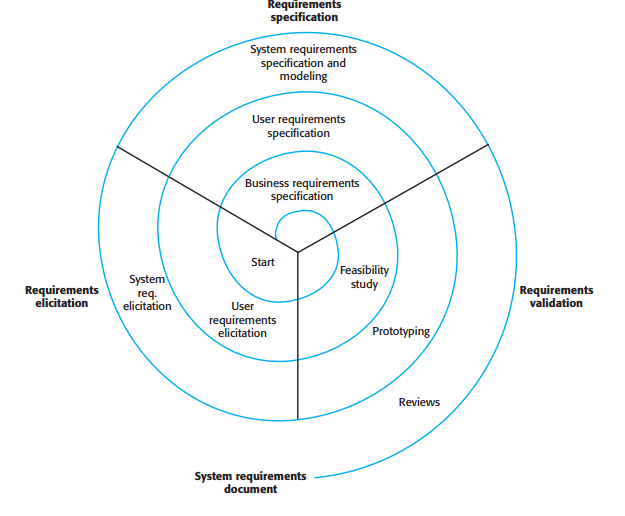
\includegraphics[width=0.80\textwidth]{Figures/spiral.png}
\caption{Spiral Model for requirements engineering (from Sommerville I. Software Engineering. Pearson, 10 edition, 2015, p. 112)}\label{fig:spiralDiagram}
\end{figure}

At the start of the project much is not known about the hardware and what requirements this produces for the project, therefore using the spiral method to slowly gain knowledge of the requirements will be a good idea. First getting the knowledge available from external sources about how the hardware can be used and also how powerful it is, and further testing this knowledge by prototyping and testing the communication between devices. 
Once the spiral method has been completed a system requirements document will have been created, and from there an adaptation of Scrum will be used.
We do not have a product owner for the project, which means that this roll for Scrum will go unused. The roll is a big part of the scrum methodology, but we deem that since there is no product owner, it is us in the group who will be explaining the requirements of the project from what we learn in the requirements engineering phase. 

Scrum makes us able to work on the project in an incremental way, and our project is actually easily separated into increments.
To give a quick example of this, the increments could be: a) establishing a connection between 2 devices, b) establishing a connection with 3 devices, where 2 of the devices cannot reach each other, and this can continue for a while.
The incrementability of the project calls for an iterative development process, which further arguments for our use of Scrum.
Another reason for us to use Scrum is also for the benefits of continuously working with shorter deadlines in the form of sprints and hopefully the last month of development will not be as stressful as it could have been.

\chapter{Implementation Plan} % (fold)
\label{cha:implementation_plan}
To implement the agile Scrum method in our project, we will be setting up a physical scrum board with columns for “Stories”, “Todo”, “Doing” and “Review”. Each row of the scrum board is to be used for the different stories in the current sprint. 

Some of the different roles needed to implement Scrum will be delegated as follows:
\vspace{-\topsep}
\begin{description}[labelindent=\parindent, labelwidth=\widthof{\bfseries The development team}, align=parright]
    \item[The Scrum master] will be assigned to a new group member at the beginning of each sprint.
    \item[The product owner] is not directly present in this implementation of Scrum, but will be represented by the entire group in collaboration.
    \item[The development team] will likewise be consisting of the entire group.
\end{description}

Every sprint will be initiated during a sprint planning meeting, where the group decides which stories from the backlog should be worked on in the coming sprint. 
A typical sprint is estimated to last one week but longer sprints may be used if needed. 

Each day typically begins with a daily Scrum meeting, where all members of the development team answers three questions: \emph{1)} What have you done since last daily scrum; \emph{2)} What are you going to work on until next daily scrum; and \emph{3)} Is there anything obstructing that. 
In this implementation of Scrum there is room for skipping daily scrums, if the group decides that it will not benefit the current work flow e.g. if no group member has finished a task and no immediate obstacles are present. 

At the end of a sprint, the group conducts a sprint review meeting, where the sprint and work of the development team is reviewed. 
This meeting is also to be closely connected with a working release of the product, but because of the structure of the project, which requires a lot of documentation and analysis in the student report, the early iterations (sprints) will not result in working releases.

% chapter implementation_plan (end)


\chapter{SWOT of Developmentprocess}
This chapter will look at the strengths, weaknesses, opportunities, and threats of using an agile development process as Scrum.
\setlist{topsep=0pt}
\vspace{-15pt}
\paragraph{Strengths}
\begin{itemize}
        \item Scrum allows to refit the requirements as new discoveries have been made. Since this project is in a new field to us as students, it is great to be flexible in the requirements as they are almost bound to change.
        \item Having a daily Scrum meeting helps spreading the information in the group so everyone knows what is going on, what are the problems with it etc, which means that better discussions in the group will occur as more people are knowledgeable of the material.
        \item Having deadlines in the form of sprints can help reduce the risk of having a very very busy scheduele close to the final deadline.
        \item Agile teams work best if the developers are in the same room for increased interactions. We are as a group fitted with just such a room.
\end{itemize}
\vspace{-15pt}
\paragraph{Weaknesses} 
\begin{itemize}
        \item We do not have a customer which is what agile methods typically rely heavliy upon, but we have to act as such amongst ourselves, deciding on what is important with good arguments for our choices etc instead.
        \item A slippery slope is saying we are doing Scrum, and not just ending up doing ad-hoc developing, where there is little sense of direction and planning.
\end{itemize} 
\vspace{-15pt}
\paragraph{Opportunities} 
\begin{itemize}
        \item It gives us opportunites to work in iterations, which can be a very nice thing when working with comples problems, seperating the problems into smaller pieces and slowly building the entire project.
        \item Agile methods gives us the opportunity to try and use something in the project, and finding its limitations as we go and thus adapting.
\end{itemize} 
\vspace{-15pt}
\paragraph{Threats} 
\begin{itemize}
        \item A lack of good documentation is a threat which is not often found in linear development.
        \item Programming the same code over and over again, because the phase of requirements engineering is not thorough enough, which can cause a lot of unnecessary work.
\end{itemize}   
\setlist{}
%Pair Programming
%Refactoring
%Versionsstyring
%Peer review (Inspection)

\chapter{Tools, Techniques and Practices} % (fold)
\label{cha:tools_techniques_and_practices}
This chapter will describe, and present a rationale for the different tools, techniques and practices, which have been chosen.
Lastly the implementation of these will be presented.
The chosen tools, techniques and practices are: \textbf{Pair Programming}, \textbf{Refactoring}, \textbf{Version control} and \textbf{Peer Review (Inspection)}.

\section*{Pair Programming} % (fold)
\label{sec:pair_programming}
\begin{description}
    \item[What?]\hfill\\
    When coding two programmers may work together on the same machine/computer.
The process involves two distinct roles; One programmer writes the code and the other reviews each line of code, as it is written. 
However the two programmers are encouraged to switch roles once in a while, during the pair programming.
    
    \item[Why?]\hfill\\ 
    Often when programming, especially if the programmers lack expertise in the field in question, pair programming can be utilised to overcome obstacles, since the second developer may have some profound idea or approach to a given problem.
    This is certainly true when it comes to a project group, where all members not only have different levels of experience, but almost everyone are working in a completely new field e.g. this semesters embedded systems.
    Moreover it is expected that every member of the group writes code, and considering the relatively small project where a completely parallel workflow is impossible because of dependencies, pair programming is the ideal solution to utilise all available labor.
    Another rationale for using pair programming is the effect is has on certain oncoming bugs.
    When a bug is encountered while writing the code it is often helpful to the programmer to explain what the code is supposed to do out load.
    This is also known as \emph{Rubber duck debugging} where a programmer explains the given code to a rubber duck, and in the process of doing this realises what may be causing the bug.
    However then pair programming this rubber duck is replaced by another developer, which often will speed up the debugging.
    
    \item[How?]\hfill\\
    As a concept pair programming is fairly easy to implement in a project group.
    It is mainly done by assigning programming tasks to pairs of people instead of just one student.
    The problem with pair programming comes when a given task is to be done at home.
    Here it is very naive to expect that two group member will coordinate their time and place in order for the pair programming be utilised.
    However certain elements of the pair programming may still be used with the consulting of another group member when an obstacle is facing the coder.
    This is not an optimal solution and often the different programming tasks are plan so that they are doable when a pair programming setup can be performed.
    Some members of the project group may not want to be part of a pair programming duo, however it is not only the coder that benefits from the process but also the observer can gain some knowledge, so one should always try to incorporate a partner into the process of writing code for the project. 
\end{description}
% section pair_programming (end)
\section*{Refactoring} % (fold)
\label{sec:refactoring}
\begin{description}
    \item[What?]\hfill\\
    When existing code is restructured and/or changed without changing the way it behaves to the user (externally), it is called refactoring.
This technique is generally used to gain readability and maintainability in a codebase.
A large part of the refactoring process can be done by almost any IDE or text editor, and consists of formatting the code to be more readable; furthermore some tools can do extensive refactoring i.e. rewriting methods and functions or catching dormant bugs.

    \item[Why?]\hfill\\ 
    Refactoring is used in our project because the benefits of having more readable and maintainable code, far surpass those of spending the extra time to refactor code.
    This readability an maintainability is especially important when working on project which involve other programmers. 
    One programmer may do things a certain way that is not easily understood by others, and by then refactoring such code during a review process or pair programming the rest of the development team can easily pick up where that one programmer left off.
    Context switching for a programmer, i.e. reading a completely new (or long forgotten) piece of code, is very slow especially when readability of the code is low; this problem can be made less significant with proper refactoring. 
    
    \item[How?]\hfill\\
    To implement refactoring in the work process of our project, the first step is to ensure that all programmers agree on how to do it.
    Refactoring has zero benefits if each programmer has a different approach and no general consensus has been made about the output of refactoring.
    After that it is important that every review process and pair programming session has extra focus on refactoring, since fresh eyes often can see certain pitfalls the original programmer may not be aware of.
    Furthermore every programmer should be encouraged to use any refactoring or formatting provided by external tools, as long as said tools does what is agreed upon in the group. 
    Too maintain a high level of refactoring is should be considered as a key concept during development, and no code should be submitted to the project without a thorough refactoring.  
\end{description}                       
% section refactoring (end)

% chapter tools_techniques_and_practices (end)
\chapter{Evaluation} % (fold)
\label{cha:evaluation}
This chapter consists of evaluations of: the development process; the consequences of the tools techniques, and practices in use; and future practices and changes that should be applied.
\myref{tab:dev-process-eval} and \myref{tab:ttandp-eval} also presents the different evaluations.
% chapter evaluation (end)   

\section{Evaluation of the Development Process} % (fold)
\label{sec:evaluation_of_the_development_process}

The elements from our development process, and version of scrum, which provided the most significant improvements to the project, were the use of a scrum board and the daily scrum meetings.
However the incorporation of a scrum board was difficult at first, because of the amount of courses the project group had to attend.
The important updating of the scrum board was also somewhat neglected at times, meaning that because of bigger tasks and user stories, some group members ended up with ad-hoc tasks which was not listed on the scrum board.
This could have been solved by analysing the different stories better and writing more explicit tasks.
Moreover the daily scrum meetings proved impractical at times, when no significant work had been done, usually due to excessive course activity or the same problem as discussed before with unfulfilling tasks for different stories.
It should be noted that generally the scrum board and the daily scrums, helped the group stay synchronised with their work, and ensured that dependencies among tasks and stories could be quickly resolved.

One of the downsides in regards to the way scrum is implemented as our development process is the lack of a product owner.
This made it difficult to decide which features to develop and especially in what order, hereby inhibiting some dependencies in the project.
Additionally the role of the scrum master could benefit from being granted more focus, which in turn would make the workflow more regulated and ordered.
Finally the group work would be strengthened if harder and stricter deadlines were applied, since the amount of work done was very minor at times.   

Furthermore, since the project group had little knowledge of embedded systems at the beginning of the project, it was very helpful to not have to plan the whole project ahead of time, and instead take the agile approach with incremental problem solving.

% section evaluation_of_the_development_process (end)
\section{Tool and Techniques Evaluation}

The use of pair programming for our project has worked well sometimes, the quality of the code is better than code written by one person, which often requires more refactoring than the code written when pair programming.
This has at least been the case for us. 
We need to be better at using pair programming as it is specified, which means that the person overlooking the other programmer should not have his own computer turned on aswell, we think this would increase the quality further. 

For version control we used git which resulted in us being able to work in parallel and just merge any conflicts if they ever occur.
We make branches and pull requests to control the workflow and making sure that any work being done using git will get peer reviewed, as it will not be pushed to the master branch unless a pull request has been made ensuring that someone has reviewed it.
Before using git we tried using Sharelatex, which is like Google Docs but uses \LaTeX, this worked okay but, our review process was lacking, therefore we decided to make the change to Github for the added functionality in using pull requests etc. 
This requires an explicit action before text is in the master, therefor forcing the review process. 

Peer review work very well for us as the quality of everything is a lot better than if we did not use it, it also helps us spreading the knowledge of all the different parts of the project, since more people will have the same parts of the project.

We also decided to review the result of previous iterations, if new requirements appear we can go back and review different parts to ensure they are up to date with the new requirements.
We delete useless things, and ensure that everyone understand everything written, which is exactly what we wanted from it.
\chapter{Evaluation of practices}
With the SOE course we have taken a close look at the processes we have used for this semester, and the ones we have adapted from our use on previous semesters.
The most notable of these is Scrum, we have used a relaxed version of Scrum, as there is not a product owner available. 
The primary advantage we had using Scrum was the Scrum board, and the mindset of (bi-)weekly sprints.
This have kept our group in sync with each other, and have kept us on the right track. 
However we have moved so far from the original Scrum model, we would like to move back closer to it.
This includes being better to have proper sprint meetings, harder deadline, and a better backlog etc. 

A significant problem in the project group have been that the elective courses have taken up a lot of time, sometimes causing the group to not do proper stand-up meetings for 2 days in a row. 
This problem was in part solved by doing work as two sub-groups, however this was not a good solution in the long run, as there can be an ``us versus them'' mentality. 

Finally we shouldn't be nervous about making big changes, especially early on, to improve the quality of our work. 
This might mean that we remove something one or more group members have spent a lot of time on, this is also why it can be hard to remove. 
However it is often the correct choice as new information is gathered, and we as a group are smarter on the subject and therefore can make better decisions.

\appendix 
\chapter{Appendix}
\clearpage
\begin{sidewaystable}[]
\centering
\caption{DANK}
\label{my-label}
\begin{tabularx}{\textwidth}{|l|X|X|X|X|}
\hline
Scrum
& How do we do this activity?                                                                                                                                                                             & Does it work?                                                                                                                                                                                                                                                                              & How do we know?                                                                                                                                                                                                                                                                                                                                                                                                                                         & How can practice be improved?                                                                                                                                                                                                                                                                \\ \hline
Daily Scrum                 
& Stand-up meeting, yesterday, today, problems?                                                                                                                                                           
& Yes, when we do it, and people take it seriously. Sometimes offtracking.                                                                                                                                                                                                                   
& In the periods where the technique is used properly, the productivity of the group has been higher, and the synchronization in the group is a lot better. We cannot show data for this, but this is the result we can feel.                                                                                                                                                                                                                             & More controlled process. A dedicated scrum master instead of a interchangeable scrummaster, should result in us following the process better.                                                                                                                                                \\ \hline
Scrum Board                 
& Physical board in group room, using post-its.                                                                                                                                                           
& Yes, however sometimes we have been bad at keeping it updated. Mainly because of people having diffirent couse schedules.                                                                                                                                                                  
& Sometimes when we had a lot of courses, it would often be outdated. 
Some of the group had one course, while the rest had another, which resulted in us not being at the university at the same time, which had the results of us not updating the physical scrum board. 
Later into the project when courses are not as intense anymore, we can see an improvement in the usage of the board, and also how it creates an image of progress for the group & Agreeing on a meeting time to actually have the daily scrum to update the scrum board, even when courses interfere. 
Some days half the group would not show in the group room due to courses.                                                                                                \\ \hline
Scrum Master                
& Scrummaster will be passed around from each sprint.                                                                                                                                                     
& No, not really, but it might be because of the very faint usage of the scrum master, which was basically just controlling the daily scrum meeting. 
And it was not always announced who was scrum master, so someone each day would control the meeting, which might have caused confusion. & The meetings are not as controlled, and the scrum board has not been used to full effect. The backlog was not used properly either, however, this is not mentioned elsewhere in the table. A proper scrum master role might results in this being followed better.                                                                                                                                                                                      & Maybe some kind of explicit indication of who the scrummaster is, could help remove potential confusion, e.g. a badge or hat of some kind. Moreover a specific set of procedures could be made available to the scrummaster, which in turn would make the role of scrummaster more tangible. \\ \hline
Product Owner               & We have not had a dedicated PO, this is the result of this being a student project without an external stakeholder. The role of the product owner has been taken by all group members in collaboration. & Yes/No, sometimes it is easy to choose what tasks to do in the next sprint, however a dedicated PO would have been very helpful at times.                                                                                                                                                  & We have no data to show how it would have been different with a dedicated PO.                                                                                                                                                                                                                                                                                                                                                                           & Either getting a dedicated PO (hard for student projects) or assigning a group member to fulfill the role each sprint.                                                                                                                                                                       \\ \hline
\end{tabularx}
\end{sidewaystable}

\begin{sidewaystable}[]
\centering
\caption{SHIT}
\label{my-label}
\begin{tabularx}{\textwidth}{|l|X|X|X|X|}  
\hline
Activities       & How do we do this activity?                                                                                                                                                                                                 & Does it work?                                                                                                                                                                                                                                                   & How do we know?                                                                                                                                                                                                                                                                                                                                                                    & How can practice be improved?                                                                                                                                                                                                                                                                   \\ \hline
Pair-Programming & When a group member takes a task which involves programming, they ask if someone wants to pair program with them.                                                                                                           & Often it does, the code produced is more thought out, than that which a single person produces. However it uses two people instead of one. Though sometimes one of the people involved would be distracted and do something else, often not project related.    & The evaluation of the code finds fewer errors in general on code which was pair-programmed. Moreover when programming in pairs, obstacles appear to be solved significantly faster.                                                                                                                                                                                                & Be more consistent about pair-programming and not getting distracted. Either by turning off electronic devices, or by physically moving away from the (loud) group room.                                                                                                                        \\ \hline
Refactoring      & When some code or text, which is unclear or “broken”, is encountered, it should be refactored if possible.                                                                                                                  & Most of the time, however the retrofitting refactoring is less used in the code base of the project because of pair programming.                                                                                                                                & It is hard to tell if refactoring works, since the code before the refactoring rarely is seen by anyone but the writer, with the exception of pair programming.                                                                                                                                                                                                                    & Everybody should be encouraged to be more aggressive in the refactoring of their own work, especially when it comes to source code. The aggressiveness should be enforced upon constructions that seems clear to the programmer but perhaps not to other developers.                            \\ \hline
Version Control  & We use Git as VC for our code, project report, UPPAAL-models and presentations. Each task is worked in a branch, after completion it is merged into the master branch.                                                      & Yes, it is for us unimaginable not to use a VCS. This allows us to seamlessly develop six people concurrently, do peer review and collect it all easily.                                                                                                        & We have frequently developed six people simultaneously, and havn’t had any issues doing peer-review and collecting.                                                                                                                                                                                                                                                                & Using better names for branches and better commit messages. This can make it easier to indentify what changes has been made by looking on Github or in your local repository.                                                                                                                   \\ \hline
Peer Review      & We peer review every time a task on the scrum board is in the “Review” column, and nothing is done before it has been through this review process. This happens for all project parts, code, tests, text for the paper etc. & It works yes, many times mistakes have been corrected using this technique. Sometimes one group member might write a section in a way the peer reviewer does not agree with, and this sparks a discussion of the contents, which heightens the quality greatly. & We know because we can see the changes on git from when a pull request is created on a task. Here the peer reviewer will look over the pull request, spell check the files, and make corrections if errors or inconsistencies are found.These bigger changes always happen in discussion with the original author, which forces us to think of why we are writing what we are etc. & This activity might suffer from the sometimes non-optimal use of the scrum board, which means some tasks might have slipped through the reviewing process now and then, however refactoring might catch these errors, but we do believe everything still in the project has been peer reviewed. \\ \hline
\end{tabularx}
\end{sidewaystable}
\endgroup

\end{document}
